\section{Introduction}
\label{sec:intro}

% Hook: The cost problem is real and urgent
LLM inference costs have emerged as a critical barrier to AI adoption. For startups, API bills can rival engineering salaries; for universities, limited research credits constrain student projects and coursework. Industry surveys report that inference costs rank among the top three concerns for organizations deploying LLMs in production~\cite{mlops_llm_survey_2023}.
Yet the common remedy---switching to cheaper, smaller models---sacrifices the quality that makes LLMs valuable in the first place.

\paragraph{The Rise of Hybrid Pricing.}
% \jason{we did not list concurrency-based provider here}.
Fortunately, the LLM marketplace has evolved beyond simple pay-per-token APIs. The commoditization of open-weight models (Llama-3, Mistral, DeepSeek-R1) means the \textit{same model} is now accessible through radically different pricing structures across 10+ providers.\cite{meta_llama3_2024,mistral7b_2023,deepseek_r1_github_2025,llama_e2e_cloud_guide} On one end, pay-per-token APIs (Together, Fireworks, DeepSeek) offer unlimited elasticity but charge per token. On the other hand, subscription-based services have proliferated with two distinct constraint types: \textit{quota-based} subscriptions, such as  Chutes.ai~\cite{chutes_pricing} that provide $S_Q$ LLM requests every day for a fixed monthly price; while \textit{concurrency-based} subscriptions like Featherless.ai and Arli AI~\cite{featherless-plans,arli-pricing} serve an unlimited number of requests but limit the number of concurrent requests to $S_C$. These subscriptions offer ``zero marginal cost'' inference up to capacity limits.
Third-party coding agents like Kilo.ai even allow users to consume their ChatGPT subscription quota within IDEs~\cite{kilo_chatgpt_blog}, demonstrating the growing ecosystem around subscription-based inference.
This pricing diversity creates an opportunity: \textbf{intelligent routing can leverage a combination of the providers to achieve a low cost}.
Unlike model distillation or quantization, which trade accuracy for efficiency, our approach achieves \textit{pure efficiency gains} by exploiting pricing arbitrage across providers serving identical models~\cite{hinton_distillation_2015,frantar_gptq_2022,dettmers_llmint8_2022}.

% \jason{need a paragraph on latency}
\paragraph{Latency Is a First-Class Constraint.}
Interactive applications impose strict latency service-level objectives (SLOs), and tail latency dominates user experience in large-scale services~\cite{dean_barroso_tail}. Critically, provider latencies are \textit{non-stationary}: Figure~\ref{fig:latency_drift} shows P99 latency fluctuating by more than 5$\times$ over time for both Meta's Llama API and OpenAI's GPT-4o-mini when serving a short prompt. This variability arises from changing queue depths, shared infrastructure, and provider-side load balancing---making static provider selection inadequate.
% Our formulation treats latency as a first-class optimization dimension: we build online latency profiles through lightweight probing, employ LP-based provider mixing to construct cost-latency Pareto frontiers, and use smart hedging to guarantee tail latency when primary providers experience delays.

\begin{figure*}[t]
\vskip 0.1in
\begin{center}
\centerline{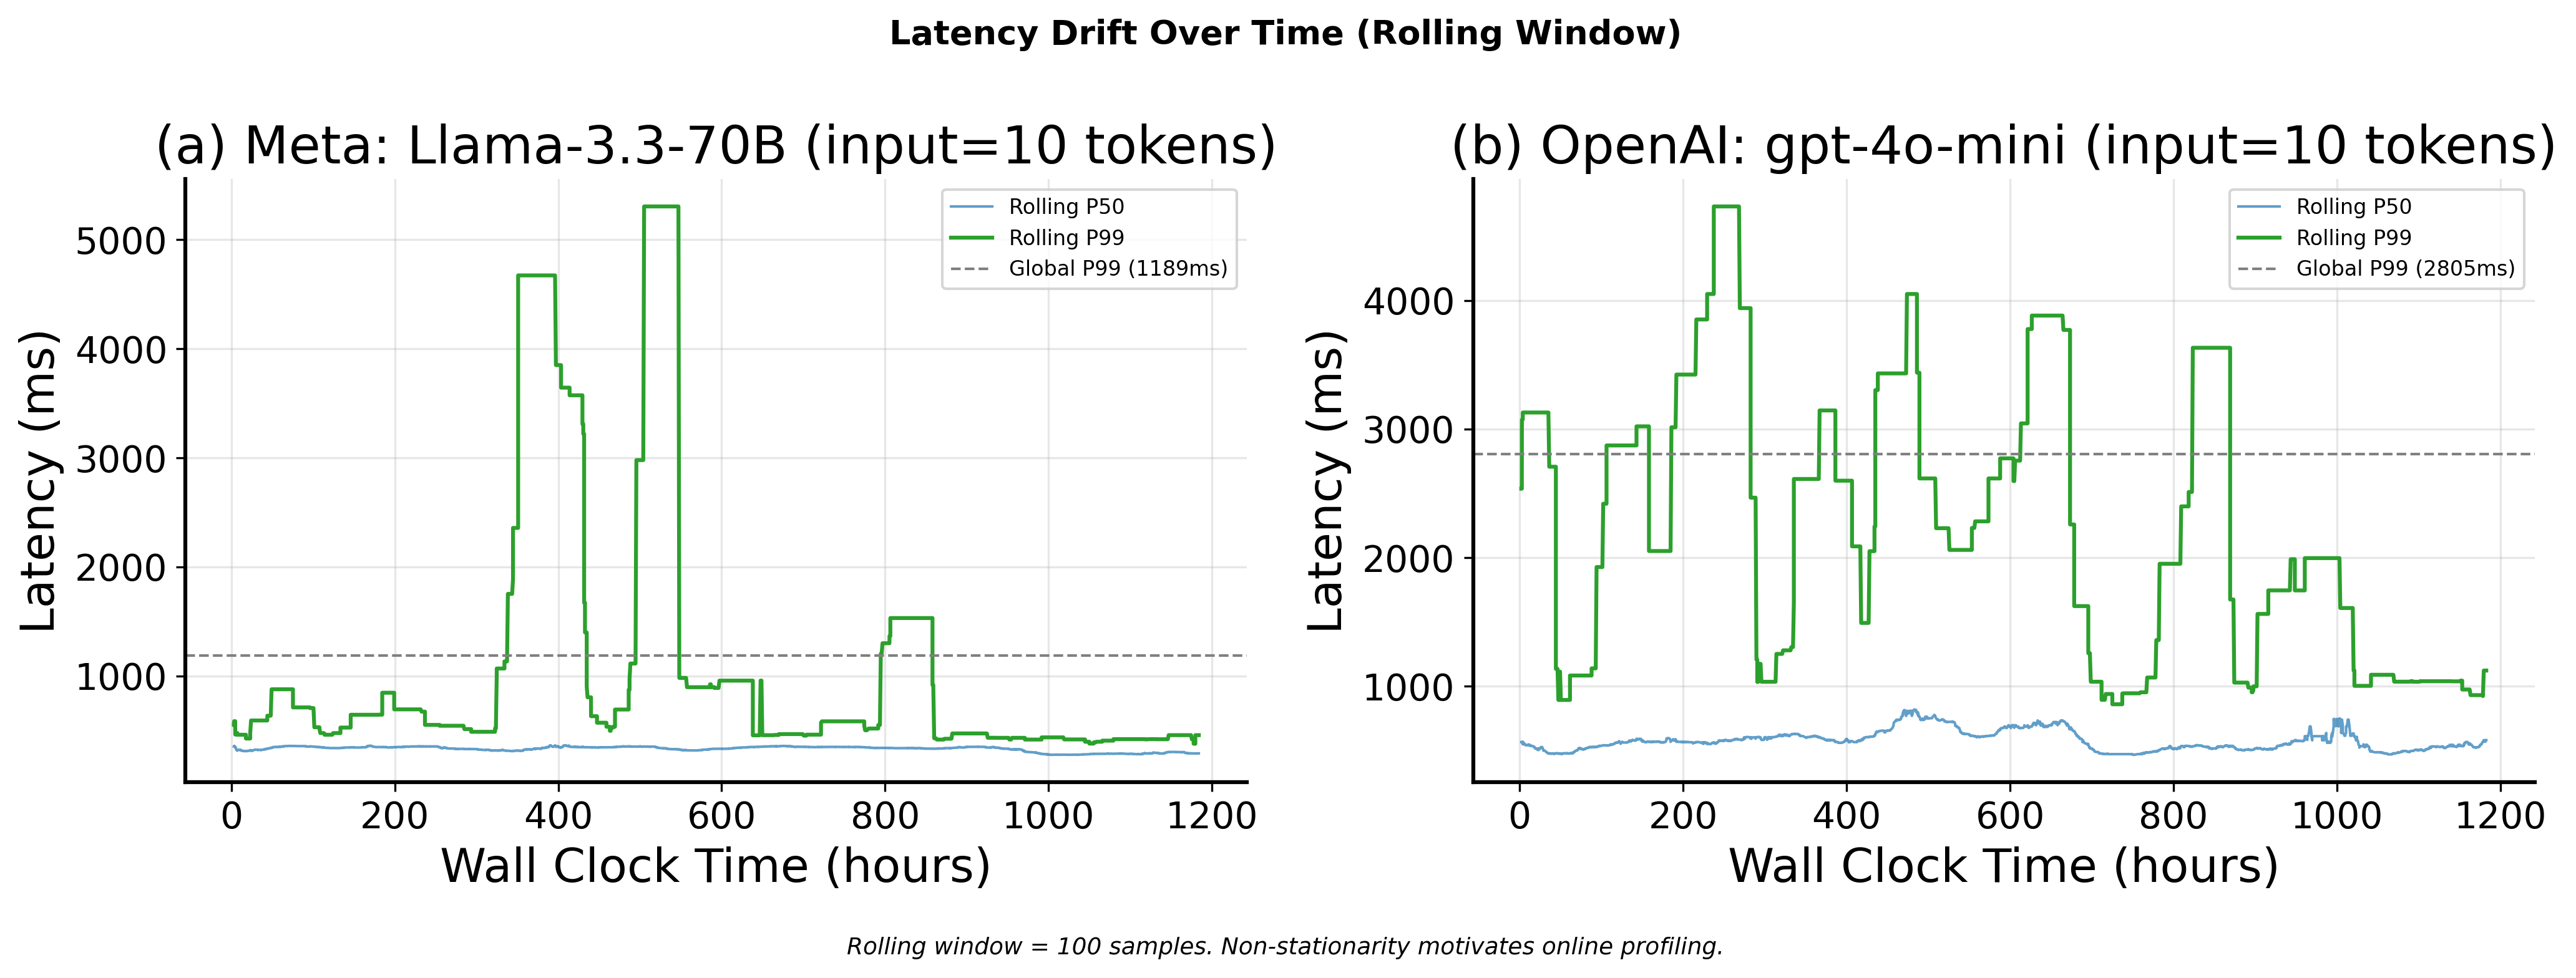
\includegraphics[width=0.95\textwidth]{images/drift_wall_clock.png}}
\caption{Provider latency over 1,200 hours. P99 latency fluctuates significantly---Meta's Llama-3.3-70B spikes from 1.2s to 5.4s, while OpenAI's GPT-4o-mini varies between 1--4.8s. The workload was collected by sending a short random prompt every 5 minutes for 50 days.}
\label{fig:latency_drift}
\end{center}
\vskip -0.2in
\end{figure*}

\paragraph{The Challenge of Opportunity Cost.}
This hybrid pricing landscape presents a classic resource allocation challenge: how to route a stream of heterogeneous requests to minimize total cost while satisfying service-level objectives (SLOs) \cite{dean_barroso_tail}. A naive greedy strategy---sending every request to a subscription until it is full---is often suboptimal. It fails to account for the \textit{opportunity cost} of consuming a scarce subscription slot with a low-value (short) request, forcing a subsequent high-value (long) request to the expensive pay-per-token API.
Consider a concrete example: a Chutes.ai subscription provides 5,000 requests per day for Llama-3.3-70B. If a user sends a trivial ``Hello'' query that would cost \$0.001 via Together API, that slot is no longer available for a complex coding request that would cost \$0.50 via API. The naive greedy policy wastes 500 $\times$ potential savings. Our experiments show that such opportunity cost losses are not merely theoretical---on real workloads, greedy routing captures only 49--83\% of the savings achievable by optimal routing (Table~\ref{tab:stage1_savings}). While motivated by the API provider marketplace, our formulation can also be applied to self-deployed GPU resource pools by modeling them as quota- and concurrency-based providers.
% \yiyan{kept one sentence here}

We address this challenge by formalizing the \textbf{Latency--Cost Optimization} problem for multi-provider LLM routing. Our contributions are:

\begin{enumerate}
    % \item \jason{add one on we categorize existing LLM inference providers into three categories, merge the first two into one} \yiyan{\textbf{Provider Taxonomy:} We categorize modern LLM inference providers into a unified set of resource types---unrestricted pay-as-you-go APIs and capacity-constrained subscriptions, where subscription constraints appear as either fixed-window quotas ($S_Q$) or reserved concurrency slots ($S_C$).}
    \item \textbf{Provider Taxonomy:} We categorize modern LLM inference providers into a unified set of resource types---unrestricted pay-as-you-go APIs ($S_A$) and capacity-constrained subscriptions, where subscription constraints appear as either fixed-window quotas ($S_Q$) or reserved concurrency slots ($S_C$).
    \item \textbf{Formal Problem Definition:} We model the routing problem under two distinct constraint types: fixed-window quotas (Stage 1) and concurrency limits (Stage 2), incorporating latency deadlines.
    \item \textbf{Offline Oracles:} We derive optimal offline algorithms for these settings. For Stage 1, we prove that a greedy-by-value strategy is optimal. For Stage 2, we formulate a time-indexed Integer Linear Program (ILP) to handle the NP-hard scheduling problem.
    \item \textbf{Online Algorithm:} We propose a Learning-Augmented Primal-Dual (LA-PD) algorithm. It uses a shadow price mechanism to value scarce resources and integrates a quantile regression model to conservatively estimate request costs under uncertainty.
    \item \textbf{Production Workload Traces:} We collect and analyze diverse LLM workloads including ShareGPT, an industry production trace, and 440K+ requests from a university campus deployment. We will release the campus trace to facilitate future research.
    \item \textbf{Empirical Results:} Using these traces, we demonstrate that our approach achieves near-optimal costs (within 1.18x of the offline oracle) and significantly outperforms standard greedy baselines.
\end{enumerate}
